%#!platex --src-specials main.tex

\chapter{提示手法比較実験}
本章では触覚提示装置を用いた心理物理実験について述べる.
我々が提案した振動提示手法を評価するために,ユーザに対してテクスチャの振動情報を
提示する実験を行った.この実験では既存手法である一次元の振動提示手法と,前章で述べた
我々が提案する二次元の振動提示手法を使用して記録振動を提示した.
また,いくつかの空間周波数が一定のテクスチャについては画像情報から得られる特徴量を
重畳した振動提示も行う.
実験協力者は本物のテクスチャと剪断力提示装置上に再現された仮想テクスチャを触り比べ,
仮想テクスチャがどの程度本物のテクスチャに類似していたかを評価する.
また類似度の評価には5段階リッカート尺度を用いた.



\section{実験内容}
\subsection{実験準備}
本実験では3.2.1節で紹介した天然芝に近いやわらかい人工芝のテクスチャ,
天然芝と異なり突起が多くチクチクした人工芝のテクスチャ,
硬めの絨毯のテクスチャ,やわらかめの絨毯のテクスチャ,
Polylactic Acid(PLA)製のタイル模様の自作テクスチャ,
目が粗くざらざらした40番の紙やすりのテクスチャ,
それぞれ材質の異なるランチョンマット3種のテクスチャ,
ツルツルした板に無数のパンチ穴が開いているテクスチャ
の10個のテクスチャを用いて実験を行った.
図\ref{5-1}に再度,実験に用いたテクスチャの画像を示す.

\begin{figure}[h]
\begin{center}
  \includegraphics[width=12cm]{texture.eps}
  \caption{実験で用いたテクスチャ}
  \label{5-1}
\end{center}
\end{figure}

また,実験協力者は22〜24歳までの健康な男性7人である.本実験中はピンクノイズを
流したヘッドホンを装着してもらい,外部の音を遮断する.さらにアイマスクで視覚も遮断する.
実験協力者は全員右利きであり,右手人差し指を用いて触察してもらった.


\subsection{実験手順}
本節では,前章で述べた提案手法と,
既存手法である一次元の振動提示手法がどれほどテクスチャを再現性高く提示できる
のかを評価してもらった.事前準備として重量計にテストテクスチャを載せてなぞってもらい,テクスチャに対する押しつけ力が50\ gf\ 程度になるように訓練してもらった.
実験の手順は以下の通りである.
\begin{enumerate}
  \item 本物のテクスチャを10秒間触察してもらい,触感を記憶してもらう
  \item ディスプレイ上に再現した仮想テクスチャを10秒間触察してもらう
  \item 仮想テクスチャが本物のテクスチャにどのくらい似ていたかを5段階評価で答えてもらう
  \item 振動提示手法を変えて再度1.~3.の手順を行う
  \item 提示テクスチャが人工芝1の場合のみ4方向の振動提示も含めて各手法3回ずつ上記の施行を行う
  \item 提示テクスチャがタイル,ランチョンマット1,プラスチックパンチの場合のみ画像特徴量を重畳する2手法の評価も行う
  \item 画像特徴量を重畳する手法については,どちらの手法がより優れていたかも二者択一で回答してもらう
  \item 自由にコメントしてもらい実験を終了する.
\end{enumerate}

なお,振動の提示手法の順番は,順序効果の影響をなくすため実験協力者ごとに
順番パターンを変えて実験を行う.実験中の様子を図\ref{5-7}に示す.

\begin{figure}[h]
\begin{center}
  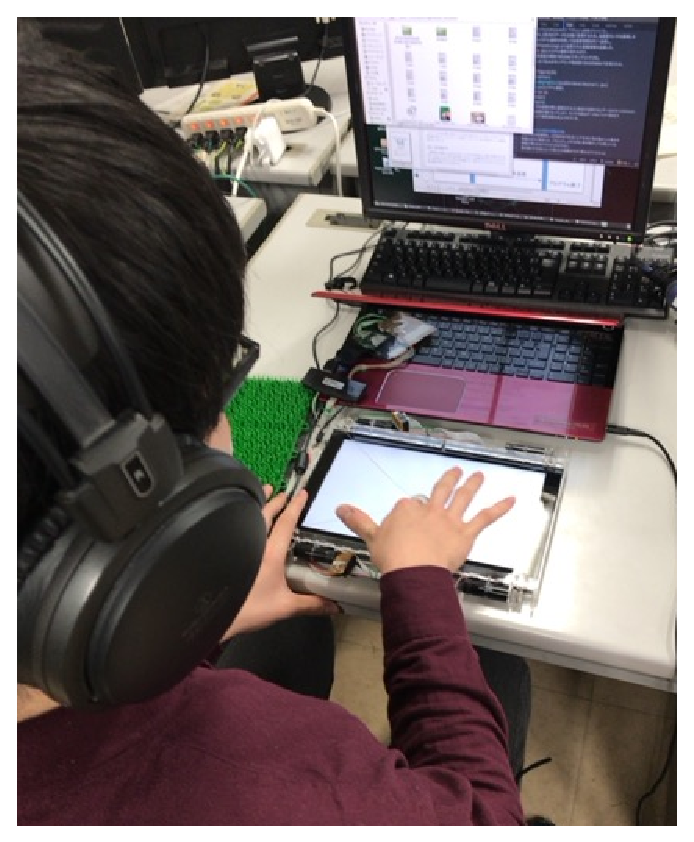
\includegraphics[width=9cm]{zikken.eps}
  \caption{実験中の様子}
  \label{5-7}
\end{center}
\end{figure}

\section{実験結果}
4.1.1節で示した10種類のテクスチャを用いて,4.1.2節の実験手順
に従い実験を行った結果を以下に示す.

\subsection{リアリティ評価実験}
テクスチャごとに各手法のリアリティを5段階で比較してもらった結果を
図\ref{5-2}に示す.
なお,分析にはTukeyの検定を用いた,図中の*は
Tukeyの検定において$\alpha<$0.05で有意な結果を示している.
\begin{figure}[h]
\begin{center}
  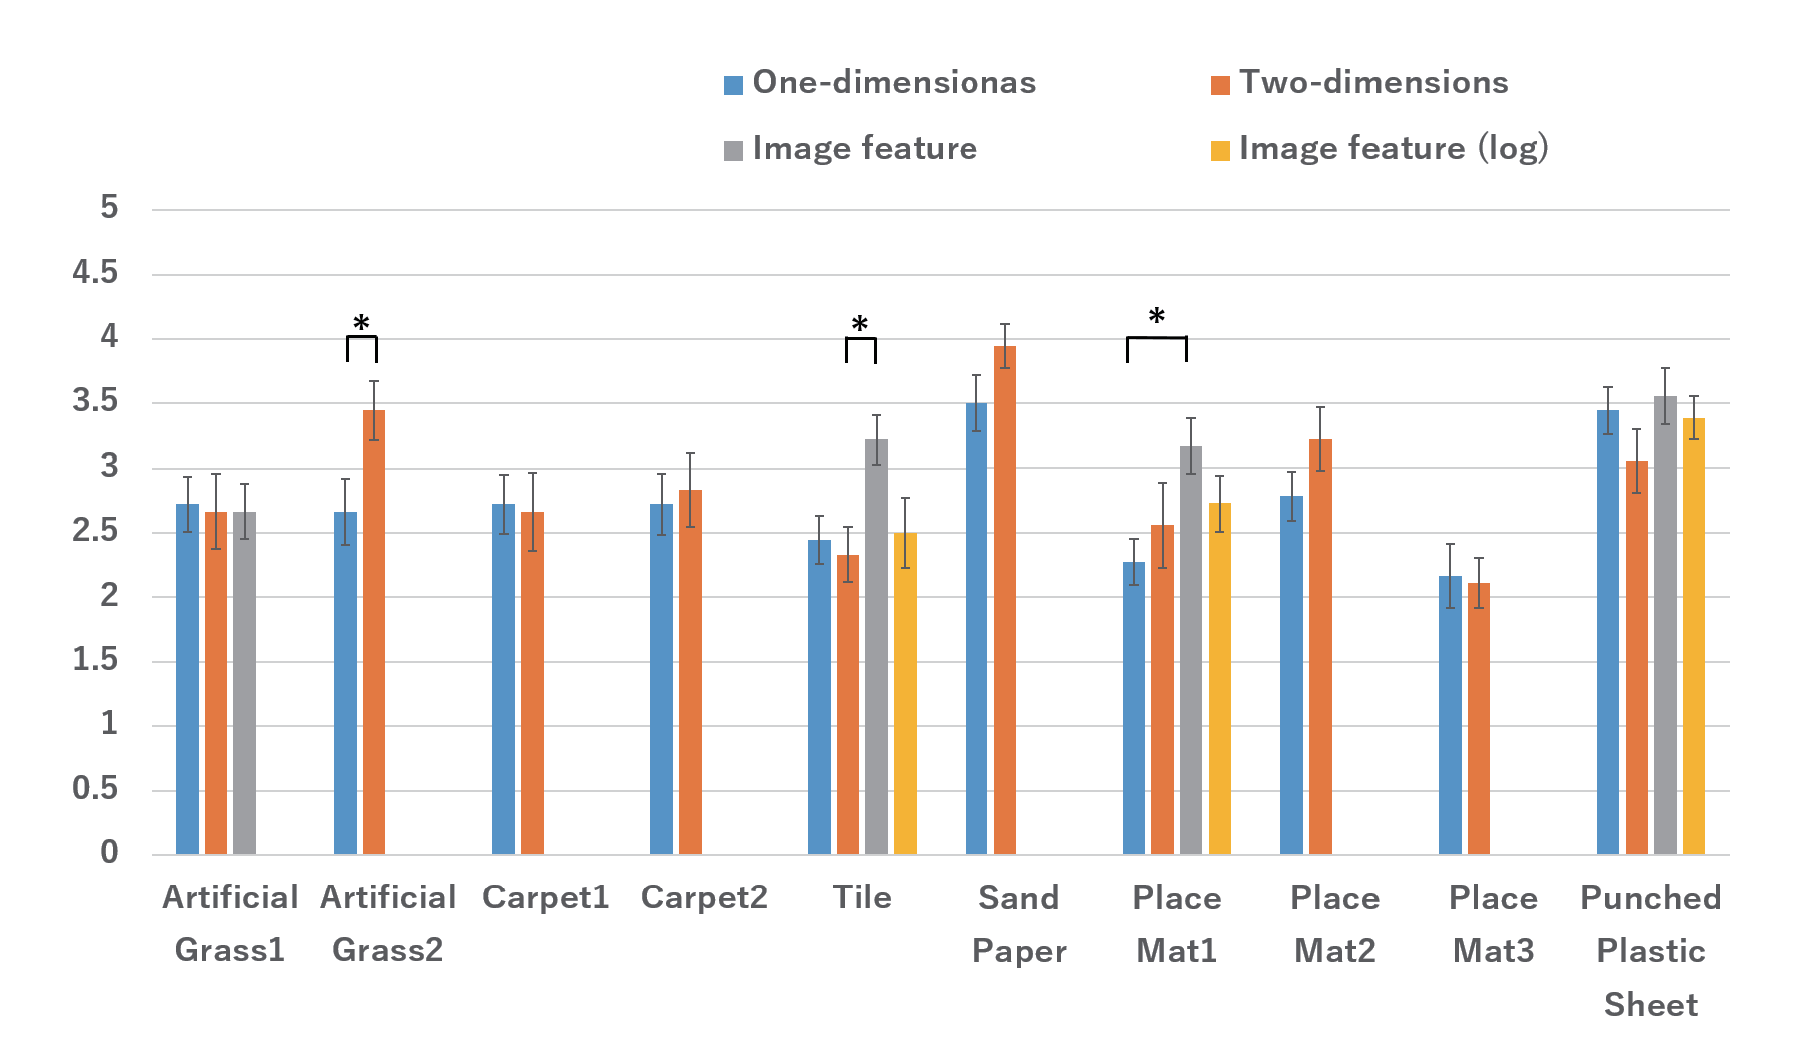
\includegraphics[width=15cm]{result1.eps}
  \caption{リアリティ評価実験の実験結果}
  \label{5-2}
\end{center}
\end{figure}
この結果より統計的に分かることを以下にまとめる.
\begin{itemize}
  \item 人工芝2では二次元の振動提示手法が一次元の振動提示手法に比べ,テクスチャのリアリティが有意に高い
  \item タイルでは対数関数を使用しない画像特徴量重畳手法が二次元の振動提示手法に比べリアリティが有意に高い
  \item ランチョンマット1では対数関数を使用しない画像特徴量重畳手法が一次元の振動提示手法に比べリアリティが有意に高い
  \item その他のテクスチャ,手法間では有意な差は認められない
\end{itemize}

\subsection{画像特徴量重畳手法の評価}
2種類の画像特徴量重畳手法について,各試行ごとにどちらの手法の方がリアリティが高いか選択してもらった結果を
図\ref{result2}に示す.

\begin{figure}[h]
\begin{center}
  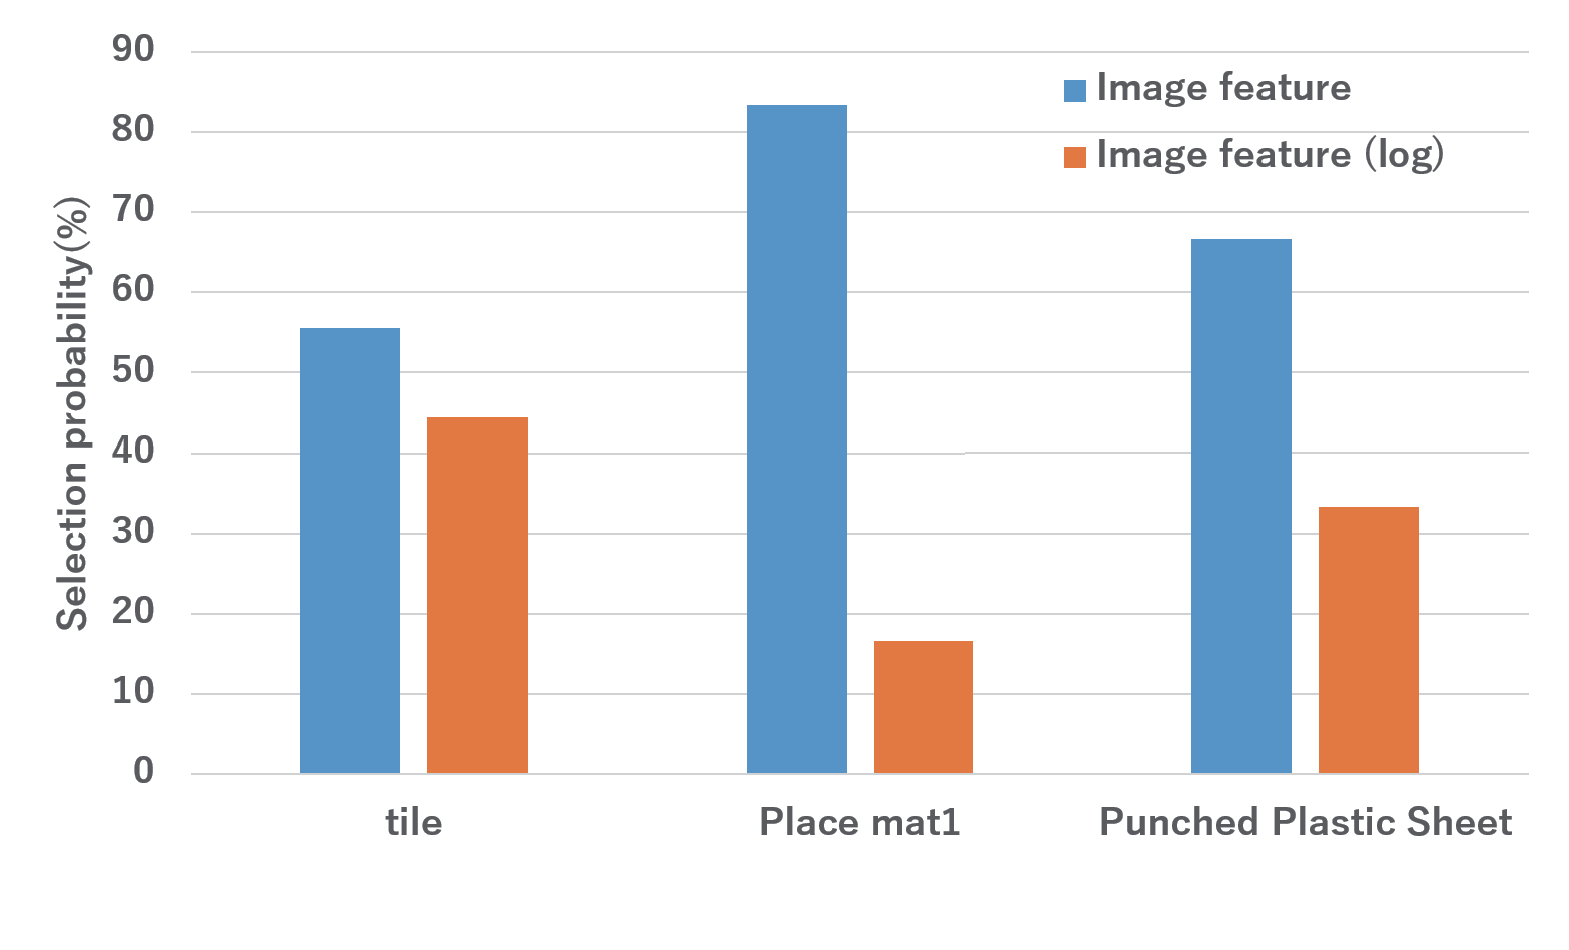
\includegraphics[width=15cm]{result2.eps}
  \caption{画像特徴量重畳手法の評価結果}
  \label{result2}
\end{center}
\end{figure}

この結果から3つすべてのテクスチャにおいて対数関数を使用せずに画像特徴量を重畳する手法の方が評価が高いという結果になった

\section{考察}
\subsection{リアリティ評価実験の実験結果}
4.2.1節の結果から,人工芝2以外では
有意差こそ得られなかったものの,我々が提案した二次元の振動提示手法
は人工芝2や紙やすり,ランチョンマット2のようなランダムな空間周波数をもつ
テクスチャに対して評価が高い傾向にあることが分かる.
この3つのテクスチャはスコアが3.0を超えており,二次元振動提示手法が
ランダムな空間周波数をもち,かつ比較的堅めの触感を持つテクスチャの
提示を得意としていると言える.
人工芝1やカーペット,ランチョンマット3といった比較的やわらかめのテクスチャ
の提示に対しては2手法間で大きな差は見られなかった.
これはディスプレイ表面が堅い素材であることなどが影響していると考えられる.
また協力者のコメントで指腹の接触面積の変化がないため評価が
低くなるといったものもあった.これは接触面積の変化によるやわらかさの知覚に
関係していると考えられる.本実験で用いた剪断力提示装置は基本的に指腹の接触面積
が一定であり,やわらかさの表現を得意としていない.そのためやわらかめのテクスチャの提示に関しては
大きな差が出なかった可能性がある.これは今後ダイナミックな振動制御などを取り入れていくことで
改善される可能性がある.  

\subsection{画像特徴量重畳手法の評価}
4.2.2節の結果から,特にランチョンマット1に対して対数関数を使用せずに画像特徴量を重畳したほうが
再現性が高くなることが分かった.このような結果になった理由として,対数関数を使用した画像特徴量の加工は振動情報の損失が抑えられる代わりに特徴点の強調が弱くなってしまうことが考えられる.
図\ref{kp}にランチョンマット1から得られた画像特徴量を,図\ref{log}に対数関数を用いて得られた画像特徴量を示す.
図\ref{kp},\ref{log}を見ても対数関数を用いた方が全体的なsizeの値が大きくなり特徴点の協調が弱くなっていることが分かる.
ランチョンマット1は特徴点間の距離が3つのテクスチャの内最も長い,つまり空間的周期が最も長いテクスチャであるため,振動強度
より特徴点の強調の方がリアリティの向上に貢献したと考えられる.

プラスチックパンチについては一定の空間周波数をもつテクスチャであるにも関わらず,二次元振動による提示でもスコアが3.0を超えて
いる.この理由としてプラスティックパンチは特徴点間の距離が短く、周期性を感じにくかった可能性がある.
つまり,一定の空間周波数をもつテクスチャでも周期が極端に短いテクスチャについては特徴量の重畳なしでも高いリアリティで提示することができる可能性が示唆された.

\begin{figure}[h]
\begin{center}
  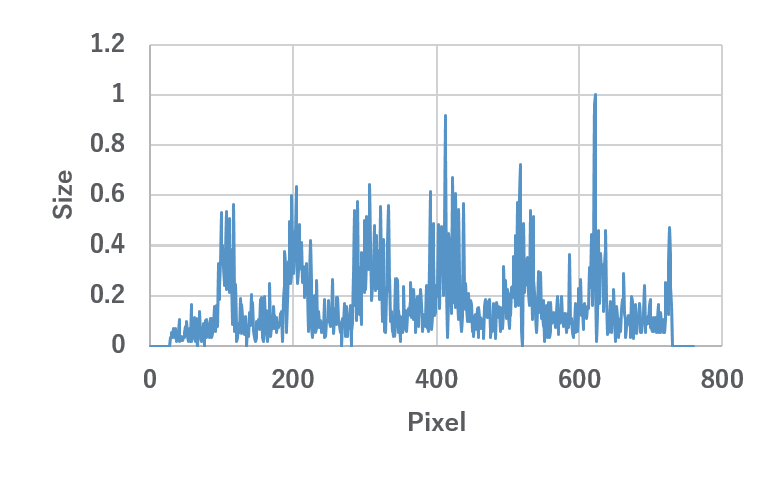
\includegraphics[width=15cm]{mat1_kp.eps}
  \caption{ランチョンマット1から得られた画像特徴量}
  \label{kp}
\end{center}
\end{figure}

\begin{figure}[h]
\begin{center}
  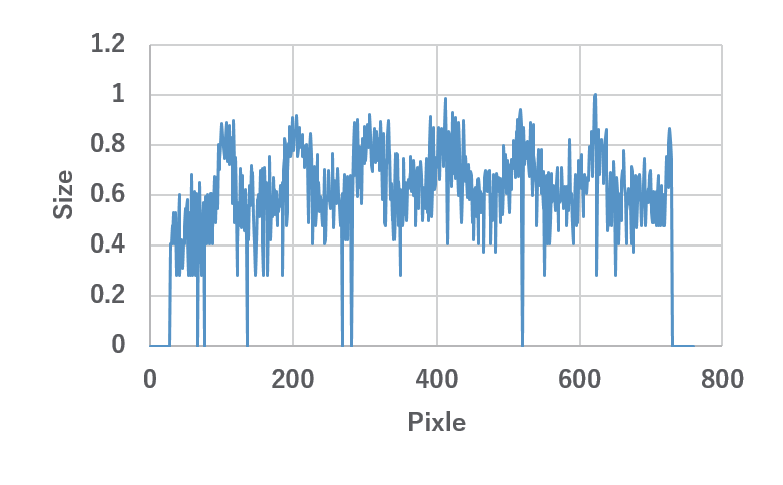
\includegraphics[width=15cm]{mat1_log.eps}
  \caption{対数関数を用いてランチョンマット1から得られた画像特徴量}
  \label{log}
\end{center}
\end{figure}


以上を踏まえ,本考察の内容を以下にまとめる.
\begin{itemize}
  \item 我々が提案した二次元方向による振動提示手法は,ランダムな空間周波数をもち比較的堅いテクスチャの提示において
,従来の一次元振動より高いリアリティで提示することができる.
  \item 比較的やわらかいテクスチャの提示においては一次元振動と二次元振動による提示手法に明確な差はない
  \item 一定の空間周波数をもつテクスチャに対しては画像特徴量の重畳を用いた振動提示手法が
より高いリアリティでテクスチャを提示できる
  \item 本実験においてはあまり有意性は見られなかったが,振動情報の損失を抑えつつ特徴点を強調できる対数関数を使用する画像重畳手法もテクスチャによっては有用である可能性がある
 \item 現在の我々の提案手法においては特徴点の強調と振動情報の損失はトレードオフの関係にあり,どちらを優先すべきかはテクスチャによって異なることが示唆された.
\end{itemize}

% Local Variables:
% TeX-master: "main"
% mode: yatex
% End:
